\documentclass[11pt]{article}
\usepackage[utf8]{inputenc}
\usepackage[T1]{fontenc}
\usepackage{amsmath}
\usepackage{amssymb} % Needed for \eth
\usepackage{graphicx}
\usepackage{geometry}
\usepackage{tikz}
\usepackage{pgfplots} % For plots
\usepackage{ulem}     % For underline, using normalem to avoid messing with \emph
\usepackage{tcolorbox} % For boxing equations if needed
\usepackage{braket}    % For QM state notation if needed
\usepackage{amsfonts}  % For \mathbb if needed

\geometry{a4paper, margin=1in}
\usetikzlibrary{positioning, arrows.meta, shapes.geometric, patterns, calc} % Added calc library
\pgfplotsset{compat=1.18} % Use a recent PGFPlots version

% Custom commands (optional)
\newcommand{\avg}[1]{\overline{#1}}
\newcommand{\prob}[1]{P(#1)}
\newcommand{\ProbDens}[1]{\mathcal{P}(#1)} % Using script P for density
\newcommand{\vect}[1]{\vec{#1}}
\newcommand{\dd}[1]{\mathrm{d}#1} % Differential d
\newcommand{\pderiv}[2]{\frac{\partial #1}{\partial #2}}
\newcommand{\deriv}[2]{\frac{\mathrm{d} #1}{\mathrm{d} #2}}
\newcommand{\muState}{\mu\text{-state}} % Microstate
\newcommand{\OmegaE}{\Omega(E)}
\newcommand{\omegaE}{\omega(E)}
\newcommand{\PhiE}{\Phi(E)}
\newcommand{\deltaE}{\delta E}
\newcommand{\ethbar}{\text{\it{đ}}} % \eth symbol for inexact differential
\newcommand{\kb}{k_B} % Boltzmann constant (set to 1 for calculations)
\newcommand{\gasR}{R} % Ideal gas constant
\newcommand{\partfn}{Z} % Partition function symbol
\newcommand{\grandpartfn}{\mathcal{Z}} % Grand partition function symbol
\newcommand{\lambdaT}{\lambda_{th}} % Thermal wavelength
\newcommand{\eps}{\epsilon}
\newcommand{\nbar}{\overline{n}} % Mean occupation number
\newcommand{\ef}{\epsilon_F} % Fermi energy
\newcommand{\kf}{k_F} % Fermi wavevector
\newcommand{\tf}{T_F} % Fermi temperature
\newcommand{\rhoeps}{\rho(\epsilon)} % Density of states per unit energy


\title{Physics 415 - Lecture 33: Degenerate Fermi Gas}
\date{April 14, 2025}
\author{} % Author not specified

\begin{document}

\maketitle
\thispagestyle{empty}

\section*{Summary}

\begin{itemize}
    \item Fermi Gas (FG): $\nbar(\eps) = \frac{1}{e^{\beta(\eps-\mu)} + 1}$ (Fermi function).
    \item Density of States (3D free particles, spin $J$, degeneracy $g=2J+1$):
    \[ \rho(\eps) = \frac{V}{4\pi^2} \left( \frac{2m}{\hbar^2} \right)^{3/2} \sqrt{\eps} \]
    Total number of particles $N = g \int_0^\infty d\eps \rho(\eps) \nbar(\eps)$.
    Grand Potential $\Phi = -gT \int_0^\infty d\eps \rho(\eps) \ln(1 + e^{-\beta(\eps-\mu)})$.
    \item T=0: $\nbar(\eps) = \Theta(\ef - \eps)$ (step function). Fermi energy $\ef = \mu(T=0)$.
    \[ \ef = \frac{\hbar^2}{2m} \left( \frac{6\pi^2 n}{g} \right)^{2/3} \quad (n=N/V) \]
    Ground state energy $E_0 = \frac{3}{5} N \ef$. Ground state pressure $p_0 = \frac{2}{5} n \ef$.
    \item T>0: Define Fermi Temperature $\tf = \ef$ (using $k_B=1$).
    Regime $0 < T \ll \tf$ is the "degenerate" Fermi gas.
    Only particles within $\sim T$ of $\ef$ participate in thermal excitation. Effective number $N_{eff} \sim N (T/\tf)$.
    Qualitative estimate for heat capacity: $E \approx E_0 + N_{eff} T \sim E_0 + N T^2/\tf \implies C_V = (\partial E/\partial T)_V \sim N T / \tf \propto T$.
\end{itemize}

\begin{center}
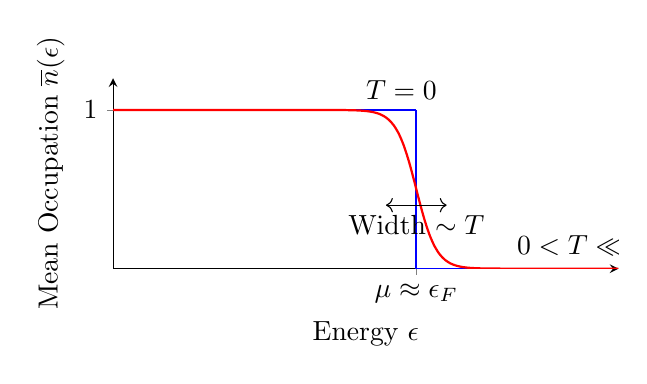
\begin{tikzpicture}
\begin{axis}[
    xlabel={Energy $\epsilon$}, ylabel={Mean Occupation $\overline{n}(\epsilon)$},
    xmin=0, ymin=0, ymax=1.2,
    axis lines=left,
    xtick = {3}, xticklabels = {$\mu \approx \epsilon_F$},
    ytick = {1},
    width=8cm, height=4cm
]
% T=0
\addplot [domain=0:3, thick, blue, const plot] {1} node [pos=0.8, above right, black] {$T=0$};
\addplot [domain=3:5, thick, blue, const plot] {0};
\draw [thick, blue] (axis cs:3, 1) -- (axis cs:3, 0);

% T > 0 (e.g., T ~ 0.1 Ef) => beta ~ 10/Ef. mu approx Ef=3.
\addplot [domain=0:5, samples=100, smooth, thick, red] {1/(exp(10*(x-3))+1)} node [pos=0.8, above right, black] {$0 < T \ll T_F$};

% Transition region width
\draw [<->] (axis cs:2.7, 0.4) -- (axis cs:3.3, 0.4) node [midway, below] {Width $\sim T$};
\end{axis}
\end{tikzpicture}
\end{center}

\textbf{Comment on Specific Heat of Metals:}
Total $C_V = C_V^{(el)} + C_V^{(latt)}$.
Conduction electrons (FG): $C_V^{(el)} = \gamma_{el} T$.
Lattice vibrations (phonons): $C_V^{(latt)} = A T^3$ (Debye $T^3$ law, derived later).
$C_V = \gamma_{el} T + A T^3$.
Experimentally verified by plotting $C_V/T$ vs $T^2$:
$C_V/T = \gamma_{el} + A T^2$. Should be linear. Holds well for many metals (see Reif Fig. 9.16.4).

\section*{Quantitative Analysis for $0 < T \ll \tf$}

We need to evaluate integrals of the form $I = \int_0^\infty f(\eps) \nbar(\eps) d\eps$ where $f(\eps) \sim \rho(\eps)$ for $N$ and $f(\eps) \sim \eps \rho(\eps)$ for $E$.
\[ I = \int_0^\infty d\eps \frac{f(\eps)}{e^{\beta(\eps-\mu)} + 1} \]
We need to evaluate this integral in the regime $T \ll \ef$ (or $\beta\mu \gg 1$), where the Fermi function changes rapidly near $\eps = \mu \approx \ef$.

\subsection*{Sommerfeld Expansion}
Introduce $\phi(\eps) = \int_0^\epsilon f(\eps') d\eps'$, so $f(\eps) = \phi'(\eps)$.
Integrate $I$ by parts: $u = \nbar(\eps)$, $dv = f(\eps) d\eps$. $du = (\partial \nbar / \partial \eps) d\eps$, $v = \phi(\eps)$.
\[ I = [\nbar(\eps) \phi(\eps)]_0^\infty - \int_0^\infty \phi(\eps) \left( \pderiv{\nbar}{\eps} \right) d\eps \]
Assume $\phi(0)=0$. $\nbar(\infty)=0$. Boundary terms vanish.
\[ I = - \int_0^\infty \phi(\eps) \left( \pderiv{\nbar}{\eps} \right) d\eps \]
The derivative $-\partial \nbar / \partial \eps = - \pderiv{}{\eps} [e^{\beta(\eps-\mu)}+1]^{-1} = - (-1)[e^{\beta(\dots)}+1]^{-2} (e^{\beta(\dots)}) (\beta) = \beta \frac{e^{\beta(\eps-\mu)}}{(e^{\beta(\eps-\mu)}+1)^2}$.
This function $(-\partial \nbar / \partial \eps)$ is sharply peaked around $\eps = \mu$ with width $\sim T$, and looks like a broadened negative delta function as $T \to 0$.

Expand $\phi(\eps)$ in a Taylor series around $\eps=\mu$ (since the peak is narrow):
\[ \phi(\eps) \approx \phi(\mu) + (\eps-\mu) \phi'(\mu) + \frac{1}{2}(\eps-\mu)^2 \phi''(\mu) + \dots \]
Substitute into the integral for $I$:
\[ I \approx \int_0^\infty [ \phi(\mu) + (\eps-\mu)\phi'(\mu) + \frac{1}{2}(\eps-\mu)^2 \phi''(\mu) + \dots ] \left( -\pderiv{\nbar}{\eps} \right) d\eps \]
Since $(-\partial \nbar / \partial \eps)$ is sharply peaked near $\mu \gg T$, we can extend the lower limit to $-\infty$ with negligible error.
\[ I \approx \phi(\mu) \underbrace{\int_{-\infty}^\infty \left(-\pderiv{\nbar}{\eps}\right) d\eps}_{=1} + \phi'(\mu) \underbrace{\int_{-\infty}^\infty (\eps-\mu) \left(-\pderiv{\nbar}{\eps}\right) d\eps}_{=0 \text{ (odd integrand)}} + \frac{1}{2}\phi''(\mu) \underbrace{\int_{-\infty}^\infty (\eps-\mu)^2 \left(-\pderiv{\nbar}{\eps}\right) d\eps}_{=\pi^2 T^2 / 3} + \dots \]
The integrals can be evaluated. $\int_{-\infty}^\infty (-\partial \nbar / \partial \eps) d\eps = [-\nbar]_{-\infty}^\infty = -(0-1)=1$.
The second integral vanishes because the integrand is odd around $\eps=\mu$.
The third integral can be shown to be $\int_{-\infty}^\infty (\eps-\mu)^2 (-\partial \nbar / \partial \eps) d\eps = \frac{\pi^2}{3} T^2$.
Thus,
\[ I = \int_0^\infty f(\eps) \nbar(\eps) d\eps \approx \phi(\mu) + \frac{\pi^2}{6} T^2 \phi''(\mu) + O(T^4) \]
Since $\phi(\mu) = \int_0^\mu f(\eps) d\eps$ and $\phi''(\mu) = f'(\mu)$:
\[ I \approx \int_0^\mu f(\eps) d\eps + \frac{\pi^2}{6} T^2 f'(\mu) \]
This is the Sommerfeld expansion (lowest order correction in $T^2$).

\subsection*{Chemical Potential $\mu(T)$}
Apply Sommerfeld expansion to the integral for $N$: $f(\eps) = g\rho(\eps)$.
\[ N = \int_0^\infty g\rho(\eps) \nbar(\eps) d\eps \approx g \int_0^\mu \rho(\eps) d\eps + \frac{\pi^2}{6} T^2 g \rho'(\mu) \]
At $T=0$, $\mu=\ef$ and $N = g \int_0^{\ef} \rho(\eps) d\eps$.
For $T>0$, expand the first term around $\ef$:
\[ g \int_0^\mu \rho(\eps) d\eps = g \int_0^{\ef} \rho(\eps) d\eps + g \int_{\ef}^{\mu} \rho(\eps) d\eps \approx N + g (\mu - \ef) \rho(\ef) \]
Substitute this into the expression for $N$:
\[ N \approx N + g \rho(\ef) (\mu - \ef) + \frac{\pi^2}{6} T^2 g \rho'(\mu) \]
(We approximate $\rho'(\mu) \approx \rho'(\ef)$ in the small $T^2$ term).
\[ 0 \approx g \rho(\ef) (\mu - \ef) + \frac{\pi^2}{6} T^2 g \rho'(\ef) \]
Let $\delta\mu = \mu - \ef$.
\[ \delta\mu \approx -\frac{\pi^2}{6} T^2 \frac{\rho'(\ef)}{\rho(\ef)} \]
Since $\rho(\eps) = A V \sqrt{\eps}$, $\rho'(\eps) = \frac{1}{2} A V \eps^{-1/2} = \rho(\eps)/(2\eps)$.
$\rho'(\ef)/\rho(\ef) = 1/(2\ef)$.
\[ \delta\mu \approx -\frac{\pi^2}{6} T^2 \frac{1}{2\ef} = -\frac{\pi^2}{12} \frac{T^2}{\ef} \]
So the chemical potential decreases slightly from $\ef$ as $T$ increases:
\[ \mu(T) \approx \ef \left[ 1 - \frac{\pi^2}{12} \left(\frac{T}{\ef}\right)^2 \right] \]
Since $T \ll \ef$, the correction is small, $\delta\mu \ll \ef$.

\subsection*{Internal Energy $E(T)$}
Apply Sommerfeld expansion to $E = \int_0^\infty g\eps\rho(\eps) \nbar(\eps) d\eps$. Here $f(\eps) = g \eps \rho(\eps)$.
\[ E \approx \int_0^\mu g\eps\rho(\eps) d\eps + \frac{\pi^2}{6} T^2 \left. [ \deriv{}{\eps} (g\eps\rho(\eps)) ] \right|_{\eps=\mu} \]
Expand the first term around $\ef$:
\[ \int_0^\mu g\eps\rho(\eps) d\eps \approx \int_0^{\ef} g\eps\rho(\eps) d\eps + (\mu-\ef) [g\ef\rho(\ef)] = E_0 + g \delta\mu \ef \rho(\ef) \]
Evaluate the derivative in the second term at $\mu \approx \ef$:
$f'(\eps) = \deriv{}{\eps} (g \eps \rho(\eps)) = g(\rho(\eps) + \eps \rho'(\eps))$.
$f'(\ef) = g(\rho(\ef) + \ef \rho'(\ef))$.
\[ E \approx E_0 + g \delta\mu \ef \rho(\ef) + \frac{\pi^2}{6} T^2 g [\rho(\ef) + \ef \rho'(\ef)] \]
Substitute $\delta\mu \approx - \frac{\pi^2}{6} T^2 \frac{\rho'(\ef)}{\rho(\ef)}$:
\[ E \approx E_0 + g \left(-\frac{\pi^2}{6} T^2 \frac{\rho'(\ef)}{\rho(\ef)}\right) \ef \rho(\ef) + \frac{\pi^2}{6} T^2 g \rho(\ef) + \frac{\pi^2}{6} T^2 g \ef \rho'(\ef) \]
\[ E \approx E_0 - \frac{\pi^2}{6} T^2 g \ef \rho'(\ef) + \frac{\pi^2}{6} T^2 g \rho(\ef) + \frac{\pi^2}{6} T^2 g \ef \rho'(\ef) \]
The terms with $\rho'(\ef)$ cancel.
\[ E(T) \approx E_0 + \frac{\pi^2}{6} g \rho(\ef) T^2 \]
Recall $E_0 = \frac{3}{5} N \ef$ and $\rho(\ef) = \frac{3N}{2g\ef}$.
\[ E(T) \approx \frac{3}{5} N \ef + \frac{\pi^2}{6} g \left( \frac{3N}{2g\ef} \right) T^2 = \frac{3}{5} N \ef + \frac{\pi^2}{4} N \frac{T^2}{\ef} \]
\[ E(T) \approx \frac{3}{5} N \ef \left[ 1 + \frac{5\pi^2}{12} \left(\frac{T}{\ef}\right)^2 \right] \]
(Note: Source has $5\pi^2/12$ factor).

\subsection*{Heat Capacity $C_V$}
\[ C_V = \left( \pderiv{E}{T} \right)_V \approx \pderiv{}{T} \left( E_0 + \frac{\pi^2}{6} g \rho(\ef) T^2 \right) \]
\[ C_V = \frac{\pi^2}{6} g \rho(\ef) (2T) = \frac{\pi^2}{3} g \rho(\ef) T \]
Substitute $\rho(\ef) = 3N / (2g\ef)$:
\[ C_V = \frac{\pi^2}{3} g \left( \frac{3N}{2g\ef} \right) T = \frac{\pi^2}{2} N \left( \frac{T}{\ef} \right) \]
This confirms the specific heat is indeed linear in $T$ for $T \ll \ef$, as argued qualitatively before.

\appendix
\section*{Appendix: Proof of Integral Result}
Prove that $I_1 = \int_0^\infty dx \frac{x}{e^x + 1} = \frac{\pi^2}{12}$.
Use geometric series for $1/(1+e^{-x}) = \sum_{n=0}^\infty (-1)^n e^{-nx}$.
\[ \frac{1}{e^x+1} = \frac{e^{-x}}{1+e^{-x}} = e^{-x} \sum_{n=0}^\infty (-1)^n e^{-nx} = \sum_{n=0}^\infty (-1)^n e^{-(n+1)x} \]
\[ I_1 = \int_0^\infty dx \, x \sum_{n=0}^\infty (-1)^n e^{-(n+1)x} \]
Swap sum and integral (assume convergence):
\[ I_1 = \sum_{n=0}^\infty (-1)^n \int_0^\infty dx \, x e^{-(n+1)x} \]
Let $y = (n+1)x$, $x = y/(n+1)$, $dx = dy/(n+1)$.
\[ \int_0^\infty x e^{-(n+1)x} dx = \int_0^\infty \frac{y}{n+1} e^{-y} \frac{dy}{n+1} = \frac{1}{(n+1)^2} \int_0^\infty y e^{-y} dy \]
The integral is $\Gamma(2)=1! = 1$.
\[ I_1 = \sum_{n=0}^\infty \frac{(-1)^n}{(n+1)^2} \]
Let $k=n+1$. $k$ runs from $1$ to $\infty$. $n=k-1$, $(-1)^n = (-1)^{k-1}$.
\[ I_1 = \sum_{k=1}^\infty \frac{(-1)^{k-1}}{k^2} = \frac{1}{1^2} - \frac{1}{2^2} + \frac{1}{3^2} - \frac{1}{4^2} + \dots \]
This is the alternating sum $\eta(2)$.
We know the Riemann zeta function $\zeta(2) = \sum_{n=1}^\infty \frac{1}{n^2} = \frac{\pi^2}{6}$.
$\eta(s) = (1 - 2^{1-s}) \zeta(s)$. For $s=2$: $\eta(2) = (1 - 2^{-1}) \zeta(2) = (1 - 1/2) (\pi^2/6) = (1/2)(\pi^2/6) = \pi^2/12$. $\checkmark$

\textbf{Euler's Proof for $\zeta(2)=\pi^2/6$}:
Consider the Taylor expansion of $\sin x$:
$\sin x = x - \frac{x^3}{3!} + \frac{x^5}{5!} - \dots$
$\implies \frac{\sin x}{x} = 1 - \frac{x^2}{3!} + \frac{x^4}{5!} - \dots \quad (*)$
Alternatively, view $\sin x$ as an infinite polynomial with roots at $x=n\pi$ ($n=0, \pm 1, \pm 2, \dots$).
We can write $\sin x$ as a product over its roots (like $P(x)=c(x-r_1)(x-r_2)\dots$). For $\sin x$, normalization requires $\sin x / x \to 1$ as $x \to 0$.
\[ \sin x = C x \prod_{n=1}^\infty (x - n\pi) \prod_{n=1}^\infty (x + n\pi) = C x \prod_{n=1}^\infty (x^2 - n^2\pi^2) \]
\[ \frac{\sin x}{x} = C \prod_{n=1}^\infty (x^2 - n^2\pi^2) \]
To match $\sin x / x \to 1$ as $x \to 0$, we need $C \prod (-\pi^2 n^2) = 1$? No.
Factor out constants:
\[ \frac{\sin x}{x} = C' \prod_{n=1}^\infty (1 - \frac{x^2}{n^2\pi^2}) \]
As $x \to 0$, the product goes to 1. So $C'=1$.
\[ \frac{\sin x}{x} = \left(1 - \frac{x^2}{\pi^2}\right) \left(1 - \frac{x^2}{4\pi^2}\right) \left(1 - \frac{x^2}{9\pi^2}\right) \dots \]
Expand this product and compare the coefficient of $x^2$ with the Taylor series $(*)$.
Coefficient of $x^2$ in product: $(-\frac{1}{\pi^2}) + (-\frac{1}{4\pi^2}) + (-\frac{1}{9\pi^2}) + \dots = -\frac{1}{\pi^2} \sum_{n=1}^\infty \frac{1}{n^2}$.
Coefficient of $x^2$ in Taylor series: $-1/3! = -1/6$.
Equating coefficients:
\[ -\frac{1}{\pi^2} \sum_{n=1}^\infty \frac{1}{n^2} = -\frac{1}{6} \]
\[ \implies \sum_{n=1}^\infty \frac{1}{n^2} = \frac{\pi^2}{6} \]

\end{document}